%\section{Redes 5G e posteriores}
\section{5G networks and beyond}
\label{sec:5G}

The evolution of mobile cellular networks has always sought to reach a ubiquitous high capacity radio, \textit{i.e.}, with increasingly lower levels of latency and higher transmission capacity. At first, the arrival of 5G adds to this evolution the opening of a path for IoT and intelligent communication technologies, exploring new forms of connectivity between Vehicles-to-Infrastructure (V2I), vehicle-to-vehicle (V2V), and Device-to-Device (D2D). However, this significant and widely publicized evolution hides the real 5G revolution, which we describe below.

5G is being developed for the innovation and evolution of cellular systems. This generation is the most dynamic and flexible mobile networks ever designed, making extensive use of cloud-native applications and network core. Moreover, 5G can shaped during its development to absorb new evolutionary leaps within the same pattern. This characteristic aims to accompany the exponential evolution of the leading technologies, such as artificial intelligence and automation. To achieve this maturity, 5G was designed to make extensive use of the virtualization of services and microservices. At first, 5G will be operated by a hybrid network, in which convergence, integration, and coexistence with legacy systems are inevitable. However, in the future, the 5G system will be predominantly composed of virtual network functions.

The 3GPP designed the 5G radio access network called Next Generation Radio Access Network (NG-RAN) and the core with a Service-Based Architecture (SBA) independently and interoperable. This is a different approach from the previous generations of mobile networks, in which RAN and core were designed in a coupled manner. Therefore, as of 5G, the standard provides for the integration of elements from different generations in different configurations. Specifically considering the transition between 4G and 5G, during the initial phase of the definition of the 5G architecture, a terminology was defined to identify the different variants that emerged from the integration between the access network and the core. The set of options are illustrated in Fig.~\ref{fig:opcoes_arq}.

\begin{figure}[htb]  
  \begin{center}
    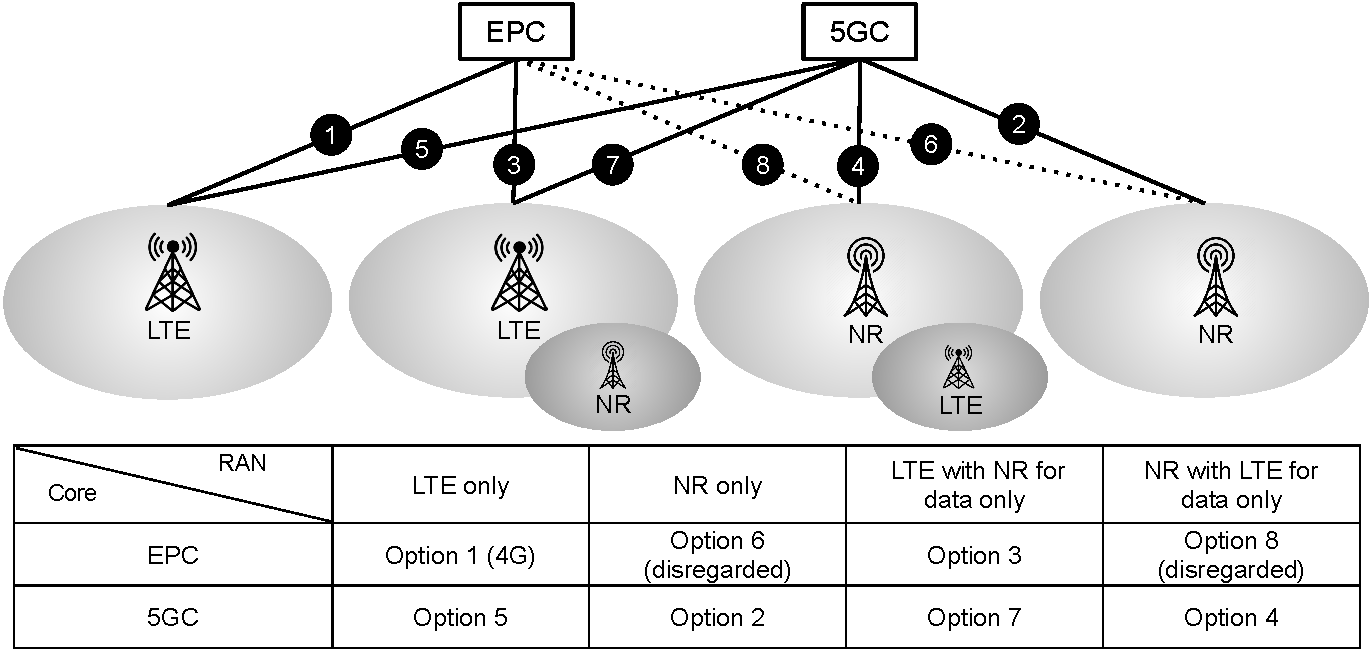
\includegraphics[width=0.45\textwidth]{figs/opcoes_arq_eng.pdf}
  \end{center}
      \caption{Options defined during the initial phase of the 5G system definition.}
 \label{fig:opcoes_arq}
 \end{figure}
 
  \begin{figure*}[htb]  
  \begin{center}
    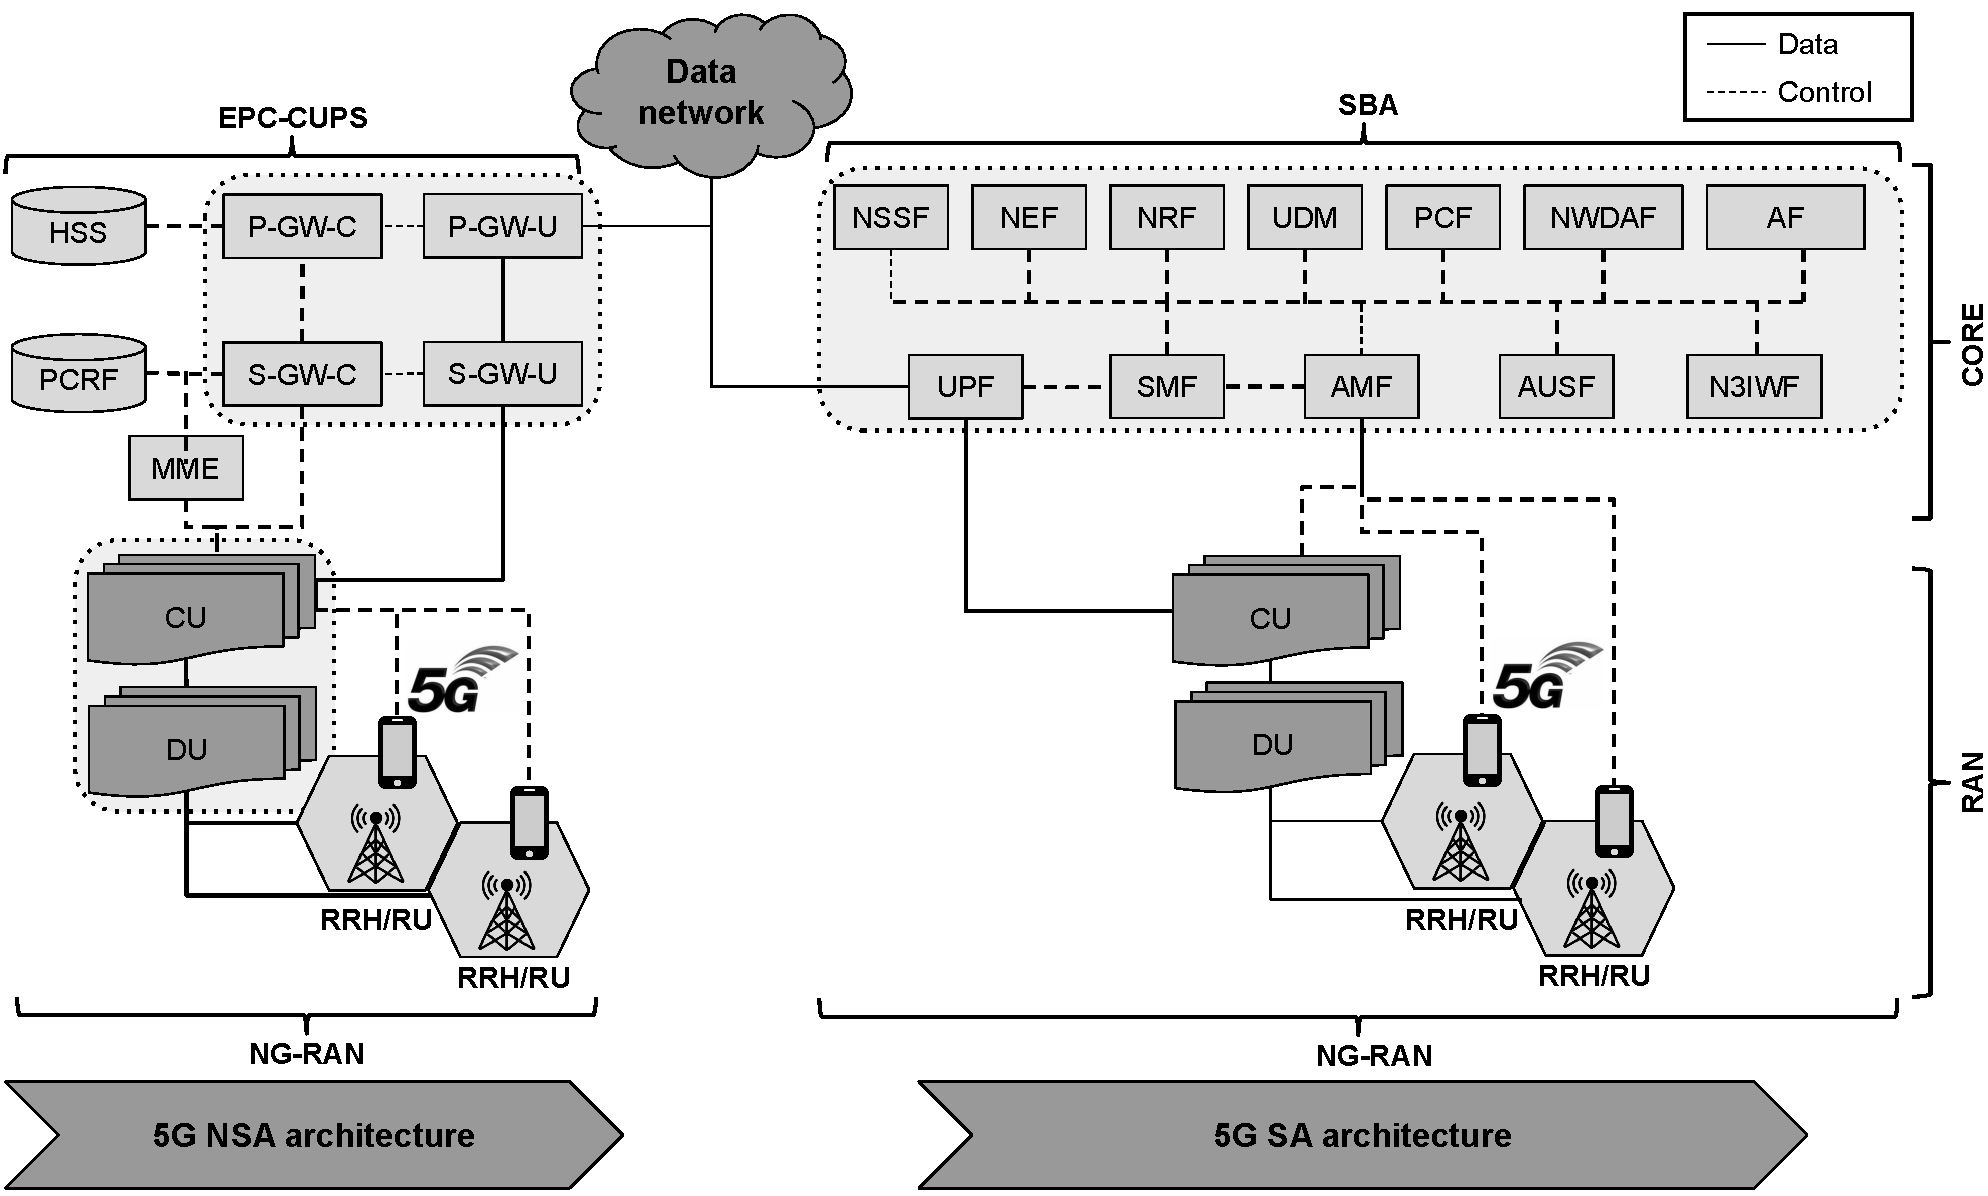
\includegraphics[width=0.8\textwidth]{figs/Arquiteturas_5G_eng.pdf}
   \end{center}
    \caption{5G architectures: Non-Stand-Alone (left) and Stand-Alone (right).}
 \label{fig:arch5g}
 \end{figure*}
In Fig. 6, option 1 corresponds to the existing 4G system and is standardized in previous releases of 3GPP. Options 6 and 8 were disregarded, as they would introduce many limitations to the 5G New Radio (NR) to provide backward compatibility with EPC. Although options 2, 3, 4, 5, and 7 were considered in the specification work, it was defined that the priorities would be options 2 and 3. Therefore, Release 15 of 3GPP introduced the Non-Stand Alone (NSA) architecture for option 3, and Stand-Alone (SA) architecture for option 2.

The NSA architecture was proposed in May 2018, and six months later, 3GPP presented the specifications for the SA architecture. NSA is a fast way to provide high data throughput and high connectivity, as it allows the use of existing network assets, without the need to implement a new complete end-to-end system for the 5G network, \textit{i.e.}, NSA is a transition architecture from 4G to 5G. In the NSA, only the radio technology needs to be updated. However, to better exploit 5G's capacity, aiming at new services, a modern architecture independent of the existing 4G system is necessary. SA is considered the ultimate 5G architecture, including improvements in radio transmission and a native 5G cloud core. The two architectures proposed in 3GPP Release 15 are illustrated in Fig.~\ref{fig:arch5g} and are discussed in the following subsections.



\subsection{5G Non-Stand Alone (NSA)}\label{sec:NSA}

The NSA architecture, also known as EN-DC (E-UTRAN-NR Dual Connectivity), meets the telecommunications industry's philosophy of introducing new technologies in the fastest and least disruptive manner. Although the motivations are clear, it is essential to highlight some disadvantages of NSA architecture. In this architecture, NR can be implemented only where 4G/LTE coverage already exists, indicating the absence of autonomy in the NSA. Furthermore, the available network functionality is limited to what is offered by LTE/EPC. Therefore, several novelties introduced in the 5G system are not available, for instance, network slicing, QoS management, flexibility in the edge computing, and the general extensibility of the 5G core, including new applications in an environment similar to the traditional cloud.

The NSA architectural design focuses mainly on allowing at least two 5G innovations to be introduced: (\textit{i}) noticeable increase in bandwidth capacity and network throughput, and (\textit{ii}) greater flexibility in the functions of the user plane provided by the gateways (S-GW and P-GW) of the EPC core. As illustrated in Fig.~\ref{fig:arq_NSA}, a separation between the control and user (or data) planes in the gateways, and a dual connection through LTE and NR are two significant features introduced in the NSA architecture. Three sets of technologies were introduced to implement these characteristics: (\textit{i}) Dedicated Core networks (DECOR) and enhanced DECOR, (\textit{ii}) CUPS and (\textit {iii}) NR as secondary Radio Access Technology (RAT). In the following, these technologies are briefly described.

 \begin{figure}[htb]  
  \begin{center}
 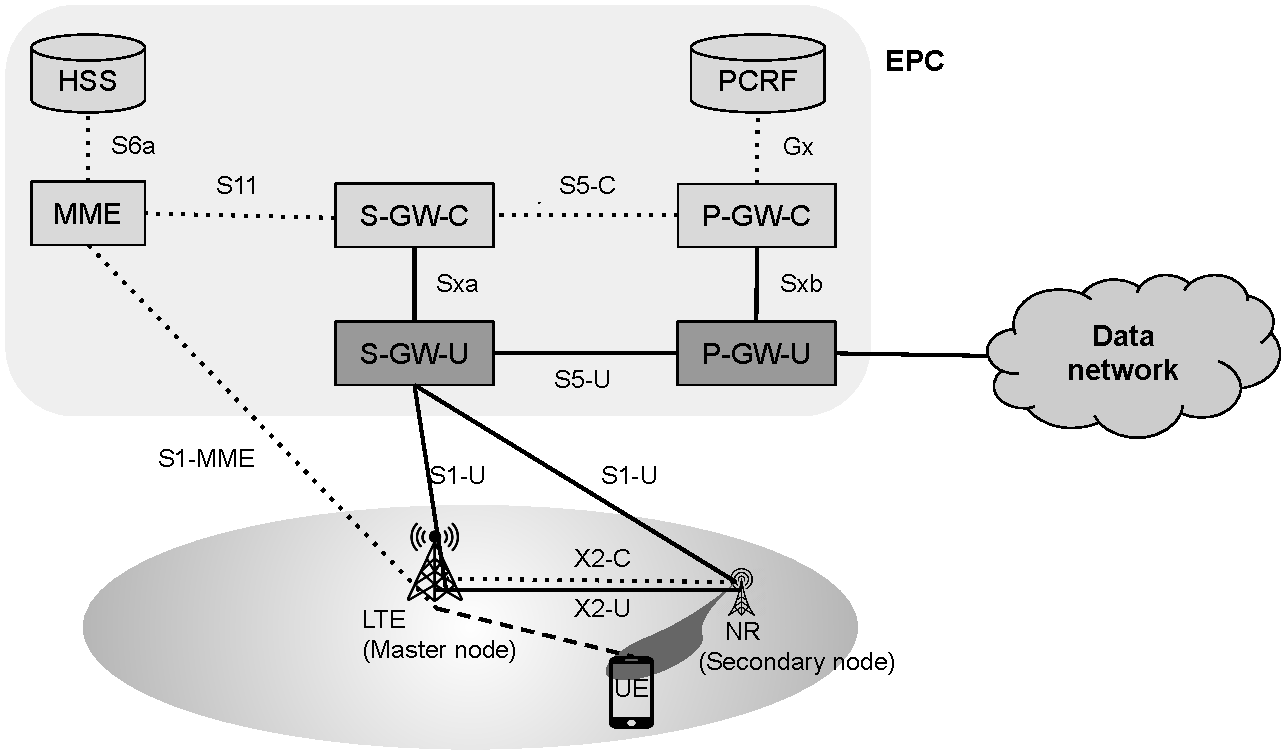
\includegraphics[width=0.5\textwidth]{figs/arquitetura_NSA.pdf}
   \end{center}
 \caption{NSA architecture, with emphasis on the selection between control and data in GWs and double connection (LTE and NR).}
 \label{fig:arq_NSA}
 \end{figure}


\subsection*{Dedicated Core networks (DECOR) e enhanced DECOR}

A mobile network operator (MNO) is recognized by its Public Land Mobile Network (PLMN) identifier, which corresponds to a mobile network core. However, even in 4G, there was a significant demand to make this approach more flexible and allow a single operator to instantiate multiple cores and direct users to the appropriate core, according to the required service. Before introducing (e)DECOR, the separation of cores was possible using different PLMN identifiers, i.e., instantiating independent core networks. An alternative solution was to use different Access Point Names (APNs) to direct users to various service networks, which were associated with multiple user plane entities, in particular, P-GWs. Both approaches, illustrated in Fig.~\ref{subfig:pre-decor}, are not flexible.

\begin{figure}[htb]
\centering
    \subfigure[pre-DECOR]
    {\label{subfig:pre-decor}
    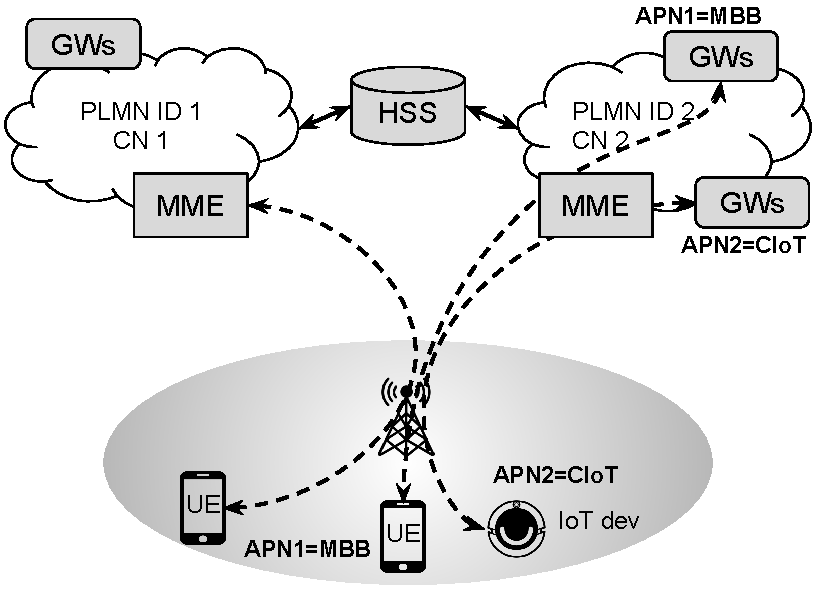
\includegraphics[width=.44\textwidth]{figs/pre-DECOR.pdf}}
    \hfil
    \subfigure[DECOR and eDECOR]
    {\label{subfig:e-decor}
    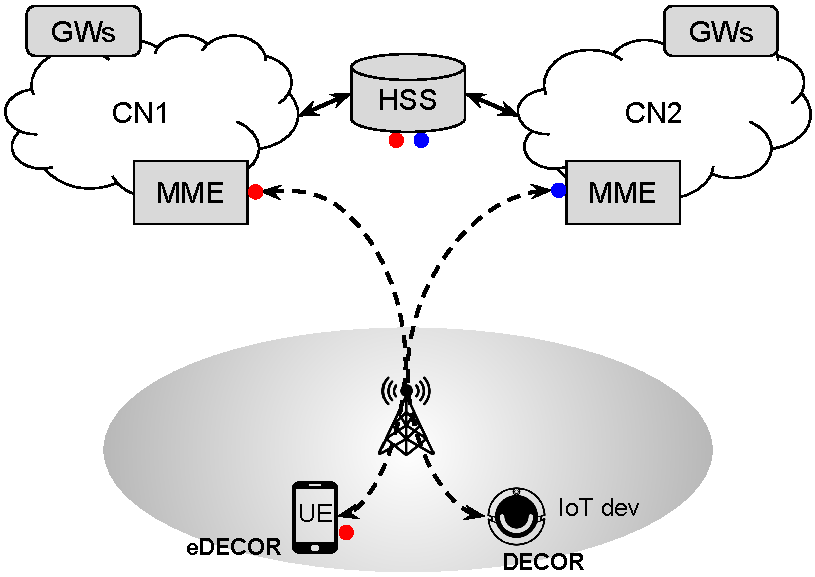
\includegraphics[width=.44\textwidth]{figs/e-DECOR.pdf}}
    \caption{Example of a pre-DECOR configuration, using APNs, compared to using DECOR and eDECOR.}
\label{fig:decor}
\end{figure}

Through the introduction of (e)DECOR, an operator can deploy multiple Dedicated Core Networks (DCNs) within a PLMN with each DCN consisting of one or more nodes of the core network (\textit{e.g.}, only MME, MME with GWs, MME, GWs, and PCRF). Each DCN can be dedicated to serving a different type of UE, separating certain types of traffic on specific core network nodes and, if necessary, adjusting them differently from the rest of the nodes of the core network. With DECOR, the information needed to identify how to route user traffic is obtained by MME by accessing only the HSS. On the other hand, eDECOR requires UE to provide specific information (\textit{i.e.}, the preferred DCN) to facilitate fast and optimal selection of the dedicated core network. Fig.~\ref{subfig:e-decor} illustrates the use of DECOR (with information initially only in the HSS, represented by the blue circle) and eDECOR (with information also in the UE, represented by the red circles) to access different DCNs.

The (e)DECOR can be considered the forerunner of network slicing, already introducing some characteristics similar to the QoS differentiation and the creation of multiple instances of some of the core components to serve different services. On the other hand, network slicing is a more advanced concept that allows the mobile network operator to perform end-to-end slicing, from the radio resources, through the entire access network and including the whole core. Network slicing should allow the creation of resource slices that are partially or totally isolated, physically, or logically.


\subsection*{Control and User Plane Separation (CUPS)}

The separation between control and user plans emerged from the need to independently dimension the user plane and control functions in the core network for session management and data services. Before the introduction of CUPS, it was not possible to deploy GW components with only the user (data) function or to independently dimension, in a standardized way, the parts of the control plane and user plane. The need for this separation became very clear as operators began to consider the impacts of third-party on their internal resources, such as (narrowband) IoT, Mobile Broadband (MBB), and also the growth of Internet-based Over-The-Top (OTT) services, such as streaming video, content sharing, and social media communication. As shown in Fig.~\ref{fig:cups}, CUPS can be applied to the following elements of the EPS: S-GW, P-GW and TDF (Traffic Detection Function).

\begin{figure}[htb]  
  \begin{center}
 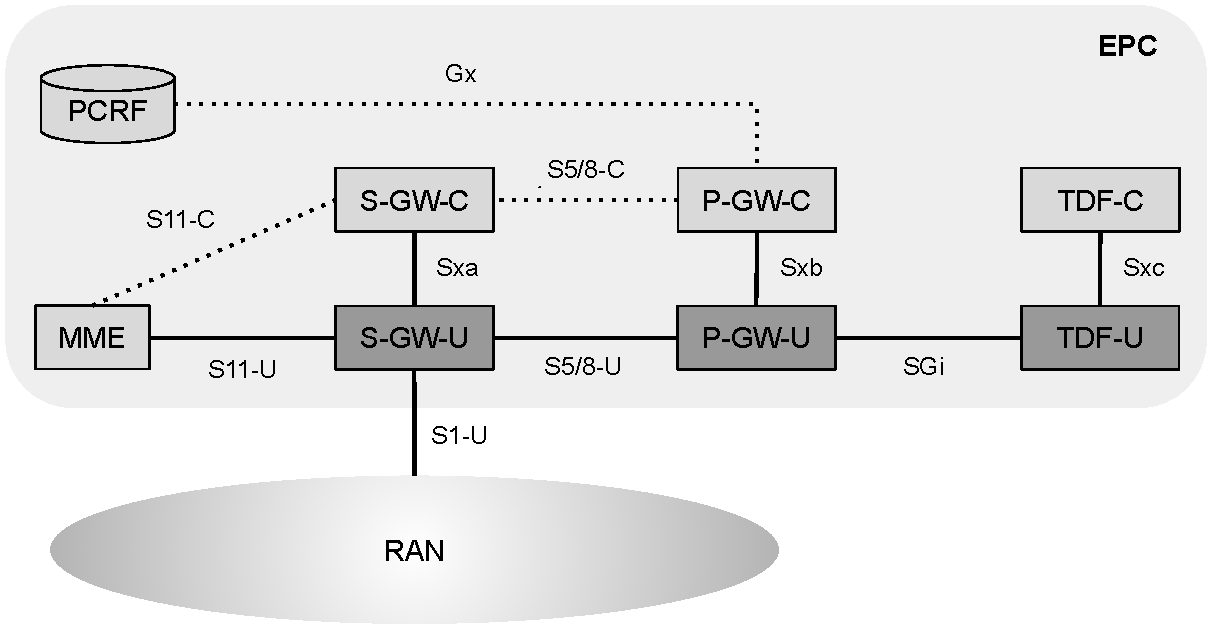
\includegraphics[width=0.5\textwidth]{figs/CUPS.pdf}
   \end{center}
 \caption{Basic EPC architecture with the separation between the control and user planes.}
 \label{fig:cups}
 \end{figure}

As shown in Fig.~\ref{fig:cups}, the control plane and the user plane of each element (S-GW, P-GW, and TDF) use an Sx interface (a, b and c, respectively) to carry out the necessary communication. The Sx interface offers procedures for establishing, modifying, and closing, thus, providing the support for the control plane and user plane operations between the components of each separated node. 3GPP standardized the Packet Forwarding Control Protocol (PFCP) to support these functionalities in Sx, and this protocol was also adopted in 5G systems.

Taking S-GW and P-GW as examples, it is interesting to highlight some design features of CUPS. It was evident that not all scenarios would require separation between the planes (control and user) and that the most common deployment scenarios would have to contemplate the coexistence of nodes with and without separation in a single network. Therefore, it was defined that the separation between the planes should not have any impact on other components of the core, such as MME, PCRF, billing system, and subscription management system. CUPS was also designed not to impact any procedure or protocol involving UEs and RAN elements. Consequently, other components of the network are unaware of whether S-GW and P-GW with which they interact have separate control and user planes or not.


\subsection*{NR as secondary access radio technology}

The dual connectivity (DC) of the NSA architecture allows UE and RAN to receive and transmit data through two base stations simultaneously. Thus, the DC provides the ability to use radio resources provided by two cells operating independently but connected to a single core. In the NSA context, the original motivation for dual connectivity is to increase user throughput, but it is also possible to provide greater mobility robustness and support load balancing between RAN nodes. Initially, the concept of dual connectivity was introduced for EPS with two groups of cells, both providing E-UTRAN resources. The BS used by the UE for initial connection (and also for all signaling with the core) is known as the master node and has the location where UE is associated. When UE reaches the connected state, the master node can request another BS (\textit{i.e.}, the secondary node) to offload data traffic. Later, the solution evolved to support multiple radio technologies (MR-DC - Multi-Radio DC), with EN-DC being the alternative that combines the technologies E-UTRAN and NR.

The requirement for spectrum flexibility was a determining factor for the adoption of OFDM-based technologies in LTE for 4G. It remains an important factor for planning and deploying NR to 5G. Throughout 3G and 4G, the need emerged for allocations in different spectrum frequency bands, several operating bandwidths, multiple duplexing schemes, and multiple-access schemes. However, the width and diversity of the spectrum used in NR represent one of the most peculiar characteristics of 5G. NR supports a large and diverse spectrum from 410~MHz to 52.6~GHz (and up to 100~GHz in future releases). Moreover, NR can use large bandwidths from 5~MHz to 3.2~GHz, supporting Time Division Duplex (TDD) and Frequency Division Duplex (FDD), as well as additional carriers for downlink (Supplementary Downlink -- SDL), or uplink (Supplementary Uplink -- SUL). In this context, 3GPP defined in the Release 15 two frequency ranges (FR): (\textit{i}) FR1 (410~MHz -- 7125~MHz) and (\textit{ii}) FR2 (24250~MHz -- 52600~MHz). FR2, also known as the millimeter-wave band, is the one that offers the greatest capacity but has different physical characteristics from FR1, presenting a challenge for deployment and use in 5G. In the following, we present some additional information about millimeter-waves, which are still a subject of significant academic interest~\cite{rangan:14, wang:18}.

In addition to being a spectral band with a low occupancy rate and less crowded, the millimeter-wave band can allow communications with rates on the order of gigabits per second, and it is quite attractive for mobile networks. However, these waves cause significant challenges in the design, implementation, and operation of these systems, as they suffer more considerable degradation and attenuation in the propagation. Moreover, these waves are more susceptible to physical blockages and atmospheric absorption. On the other hand, with the development of increasingly smaller antenna elements, thanks to its shorter wavelengths, the construction of antenna sets for the use of massive MIMO and beamforming is enabled, which helps in dealing with the propagation problems and improves significantly the frequency reuse and the spectral efficiency. However, beam forming/maintenance takes a considerable amount of time, and its improvement has been the subject of several studies~\cite{giordani:19, zhang:19}. Additionally, the problem becomes particularly challenging when considering the mobility of the users.


\subsection{5G Stand Alone (SA)}\label{sec:SA}

In the SA architecture, EPC is replaced by SBA (described in detail in Section~\ref{sec:core}), allowing the use of a set of virtual network functions that help other functions in the architecture or even for final users applications. In this way, an SA architecture consolidates the concept of decoupling of the data and control planes, allowing flexible and stateless positioning of virtual environments in the different network segments that make up a 5G system. For example, these segments can be seen as Edge, Fog, and Cloud, or even specifically in the RAN, we can find organized like Fronthaul, Midhaul, and Backhaul.

A significant evolution in the SA architecture is the design based on virtual network functions according to cloud's native model. This approach refers to how the functions of virtual networks are created and deployed flexibly, widely using the concept of cloud computing to develop, deploy, and manage services. For example, within this approach, the concept of microservices can be used for the implementation and expansion of a 5G system, in line with the fast evolution of information technology. One of the objectives of using microservices is to be able to decompose the components into functions used, with low granularity, to make the service light and with a high capacity for sharing. This objective perfectly fits the need to define eMBB, mMTC, and URLLC communication scenarios since it offers modularity, reuse of functions, and interoperability with heterogeneous networks. Furthermore, the introduction of microservices and interfaces to access them simplifies the processes of updating and maintaining 5G systems, reducing the cost of operation, and accelerating the introduction of new services.

The full implementation of SA architecture presents some challenges. For example, historically, the mobile network generations are strongly affected in the context of UE sessions, featuring a state-based architecture. On the other hand, systems based on the native cloud computing model have a fundamental feature, stateless architecture, where the contexts of their states are saved in the databases. For instance, the SBA core has introduced an unstructured data storage function (UDFS) to control the setting of network functions, as can be seen in Fig.~\ref{fig:stateless}. This characteristic allows the system to enjoy benefits such as elasticity and dynamic management of microservices on mobile networks. One of the great challenges of 5G is to design and develop software components originally based in states, through the stack of protocols used by 3GPP, for stateless microservices, enjoying the benefits of using the native cloud computing.

\begin{figure}[htb]  
  \begin{center}
 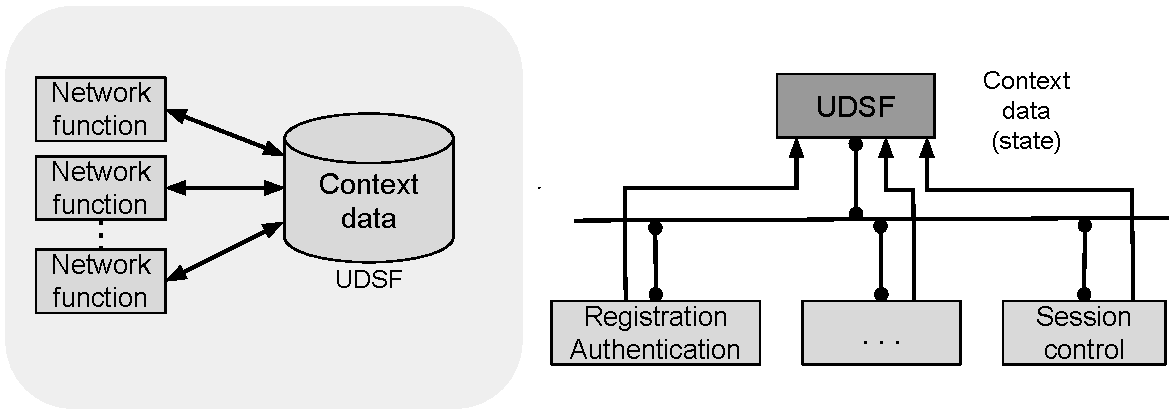
\includegraphics[width=0.5\textwidth]{figs/stateless_eng.pdf}
   \end{center}
 \caption{Context data function of SA architecture.}
 \label{fig:stateless}
 \end{figure}

In the SA architecture, the fundamental characteristic is that the elements are defined as network functions, which provide services to other functions, or any other authorized \textit{consumer}, through programming interfaces. In this way, the architecture provides extensive modularization and reusability in complete isolation between DP and CP. Due to this high modularization, the eventual migration of the NSA architecture to SA must be hidden to the end-user. Moreover, it is worth mentioning that NSA and SA are not competing for each other, but rather an evolutionary path for adopting the innovations introduced by 5G. The intention is to start with the NSA and gradually migrate to SA over time, especially for operators that already have significant investment in 4G networks. For some time, NSA and SA must coexist, and several approaches are possible. Fig.~\ref{fig:NSAeSA} illustrates a potential solution proposed by Samsung~\cite{samsung-2019}, in which an intermediate architecture emerges, using a common core.\\
\\
\textbf{Open-source software initiatives in 5G}\\
The OpenAirInterface Software Alliance also has initiated the development of software for 5G\footnote{\url{https://gitlab.eurecom.fr/oai/openairinterface5g}} involving both RAN and core. Nowadays, only basic features are available~\cite{kaltenberger:19}, but it is possible to observe the evolution of the new gNB and the 5G-NR. An operational 5G core from the OpenAirInterface is still not available, but there are efforts in several components, such as AMF, SMF, UDM, AUSF, and UPF\footnote{\url{https://www.openairinterface.org/docs/workshop/8_Fall2019Workshop-Beijing/Training/2019-12-03-NGUYEN-DU.pdf}}. Another initiative is the free5GC\footnote{https://www.free5gc.org/}, an open-source project focused on implementing the 5G core network (5GC) defined in 3GPP Release 15 (R15) and beyond. The code is organized in stages, in which stage 1 is actually an EPC implementation improved with AMF, SMF and UPF. Stages 2 and 3 are `pure' 5G core implementations, in which the latter is the most functional one. Yet another initiative is the Open Core Network group\footnote{\url{https://telecominfraproject.com/open-core-network/}} that still does not have any software available, but that is supported by the Telecom Infra Project (TIP). TIP has been involved in several other open-source initiatives related to the telecommunications industry.

\begin{figure}[htb]  
  \begin{center}
 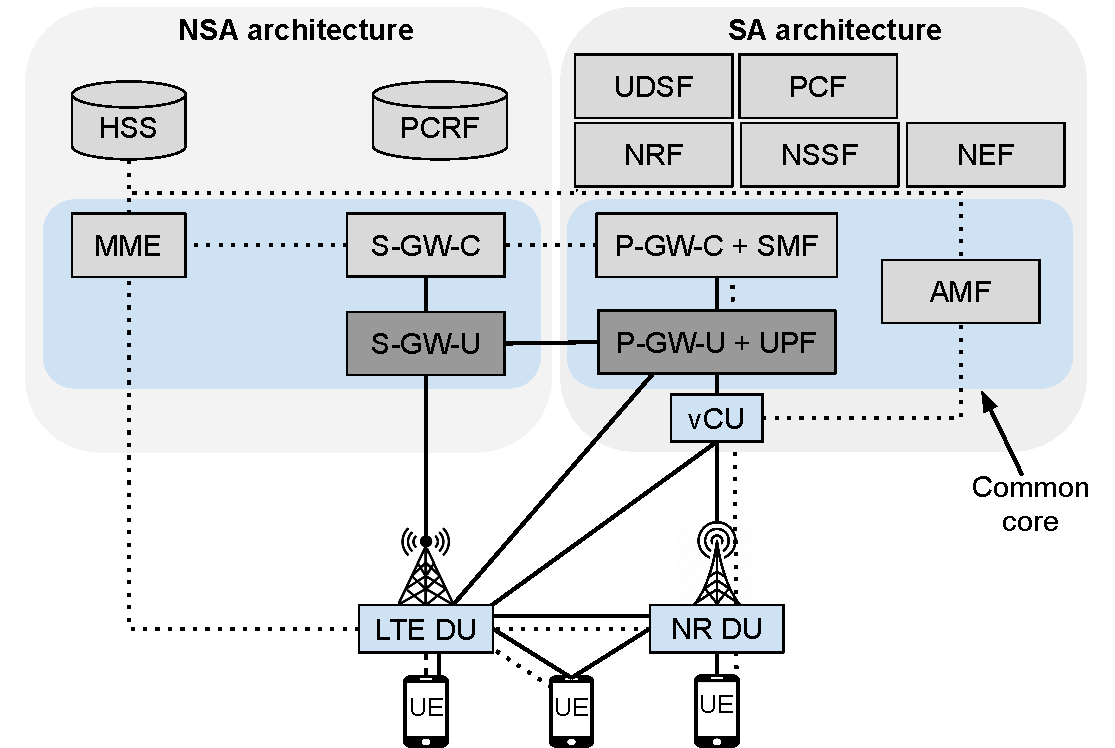
\includegraphics[width=0.5\textwidth]{figs/arquitetura_Intermediaria_eng.pdf}
   \end{center}
 \caption{Proposal for the coexistence of NSA and SA architectures.}
 \label{fig:NSAeSA}
\end{figure}


\subsection{Beyond 5G}

Although many countries, such as Brazil, are still discussing and preparing for the deployment of 5G networks, 2019 is the year when effective adoption began in several countries. Germany, China, South Korea, United States, Finland, and the United Kingdom are examples of countries that are already deploying, testing, and effectively using 5G networks. As expected, the scientific community has already begun to investigate questions 1) about the limits of 5G networks, 2) about the (new or existing) applications that would benefit from wireless communication, but would be supported by 5G networks, 3) about the technologies that need to evolve or be created to meet new potential demands, among several other themes~\cite{saad:19, giordani:20}. Although it is not possible to predict precisely what the next generation of mobile wireless networks will be and which applications will justify its adoption, but some topics are recurrent in the initial discussions and investigations and are likely to be part of the evolution of 5G networks. Among these themes are related with the efficient allocation of diverse resources in wireless networks (\textit{e.g.}, sub-6GHz bands, millimeter-waves and, in the future, bands in THz \cite{chen2019survey}), wide use of machine learning and artificial intelligence, and applications that are not served by 5G networks, such as multisensory extended reality and wireless brain-computer interactions.

5G networks have made the need to consider multiple types of wireless resources notable, in addition to the traditional licensed sub-3GHz bands. In 5G networks, it is possible to use the 3.5GHz band, unlicensed 5GHz band, millimeter-waves, and D2D communications. Additionally, there are already Multi-access Edge Computing (MEC) resources that allow improving the communication of the devices through various strategies such as caching, downloading of processing, use of context information, allocation of bandwidth, among others. However, a reliable high-band offer using millimeter-waves (later from the THz band) in mobile scenarios is a challenge that will hardly be overcome on a large scale in 5G networks. Due to the high directionality of the millimeter-wave beams, the alignment between the antennas of mobile devices and BSs must be remade with high regularity. Currently, this means disruptions in communication, but as the number of BSs (both millimeter-waves and sub-6GHz) grows, it is possible to mitigate the problem through the appropriate resources allocation policies. However, this allocation is challenging, as it involves multiple devices, multiple BSs, different resources, and must be performed dynamically in short time scales to meet the mobility of users~\cite{semiari:19}. Based on this context, there is a large amount of data that needs to be processed quickly for decision-making regarding resource allocation.

In addition to optimization models, the context described can also make extensive use of machine learning and artificial intelligence techniques. These techniques were initially explored at 4G through the concept of Self-Organizing Networks (SON)~\cite{peng:13}. In 5G networks, machine learning and artificial intelligence should have broader use, given the large volume of data to be manipulated and the greater complexity of the network~\cite{saad:19}. However, widespread adoption is expected only after the consolidation of 5G networks and in the next generation of mobile communications~\cite{letaief:19}. Moreover, the increase in the volume of data and the complexity of the infrastructure and recent evolution in machine learning and intelligence techniques have motivated its more extensive use. However, for artificial intelligence-based solutions to be widely used in communication networks, they must be built from the perspective of Explainable Artificial Intelligence (XIA)~\cite{adadi:18}. Understanding the behavior of solutions based on artificial intelligence is an essential requirement for its adoption in communication infrastructures.

5G networks are introducing new communication technologies to serve a wide range of applications and services. For example, eMBB, URLLC, and mMTC are part of the 5G system to support applications such as 4K and 8K videos, autonomous cars, virtual and augmented reality, and Industry 4.0. However, applications are already emerging that are not adequately served by 5G networks, such as multisensory extended reality, holographic telepresence, wireless brain-computer interactions, and connected autonomous and robotic systems~\cite{saad:19, giordani:20}. In general, these applications have new QoS requirements that can motivate the introduction of new classes of service such as Mobile Broadband
Reliable Low Latency Communication (MBRLLC) and Massive Ultra-Reliable Low Latency Communications (mURLLC -- massive URLLC). On the other hand, to exploit the available resources more efficiently, it is vital to investigate and adequately characterize the demand for applications, taking into account QoS requirements, Quality of Experience (QoE), and quality of Physical Experience (QoPE)~\cite{saad:19, taleb:19}.